\documentclass{article}
\usepackage{graphicx}       % Required for inserting images
\usepackage{hyperref}       % hyperlinks
\usepackage{url}            % simple URL typesetting
\usepackage{booktabs}       % professional-quality tables
\usepackage{amsfonts}       % blackboard math symbols
\usepackage{nicefrac}       % compact symbols for 1/2, etc.
\usepackage{microtype}      % microtypography
\usepackage{xcolor}         % colors
\usepackage{lmodern}
\usepackage{graphicx}
\usepackage{float}
\usepackage[acronym]{glossaries}
\makeglossaries

% Acronym definitions
\newacronym{ai}{AI}{Artificial Intelligence}
\newacronym{ml}{ML}{Machine Learning}
\newacronym{svm}{SVM}{Support Vector Machine}
\newacronym{qsvm}{QSVM}{Quantum Support Vector Machine}
\newacronym{qml}{QML}{Quantum Machine Learning}
\newacronym{pca}{PCA}{Principal Component Analysis}
\newacronym{macd}{MACD}{Moving Average Convergence Divergence}
\newacronym{ema}{EMA}{Exponential Moving Average}
\newacronym{rsi}{RSI}{Relative Strength Index}
\newacronym{atr}{ATR}{Average True Range}
\newacronym{lstm}{LSTM}{Long Short-Term Memory}
\newacronym{ann}{ANN}{Artificial Neural Network}
\newacronym{qubo}{QUBO}{Quadratic Unconstrained Binary Optimization}
\newacronym{qsvc}{QSVC}{Quantum Support Vector Classifier}

\title{The Use of Quantum Support Vector Machines for Stock Price Prediction}
\author{Ben Muir and Hasan Fakih}
\date{April 8th 2025}

\begin{document}

\maketitle
\section{Introduction}

\subsection{Context}

Quantum computing has emerged as a promising tool for solving computationally intensive problems, including those found in financial modeling. In recent years, financial institutions have increasingly turned to \gls{ai} and \gls{ml} techniques to perform predictive analytics on stock market data \cite{Xia24}. Among classical \gls{ml} models, \gls{svm}s have demonstrated solid performance for classification tasks such as stock movement direction \cite{Chhajer22}. However, \gls{svm}s encounter limitations when dealing with high-dimensional or non-linearly separable data.

\gls{qsvm}s, a quantum version of classical \gls{svm}s, exploit the properties of quantum mechanics like superposition and entanglement to enhance classification capabilities and computational efficiency. These models leverage quantum feature spaces and quantum kernels to transform classical datasets into forms that can be more efficiently classified on quantum hardware or simulators \cite{muir2025}. Furthermore, research has shown that quantum-enhanced models, particularly \gls{qsvm}s, have the potential to outperform classical models in specific financial contexts, particularly when paired with dimensionality reduction and robust feature engineering \cite{srivastava2023}.

\subsection{Problem Statement}

Stock price prediction remains one of the most complex challenges in financial analytics due to the highly volatile nature of stock market data. Classical \gls{ml} models struggle to maintain accuracy when scaling across large datasets with multiple correlated indicators. The primary objective of this project is to evaluate the effectiveness of \gls{qsvm}s for binary classification of stock price movement, using real market data and derived indicators. A secondary objective is to test whether the quantum model can achieve competitive or superior performance compared to existing models.

\subsection{Result}

This project successfully implements a \gls{qsvm}-based classification system using Qiskit's quantum machine learning library. The system is tested across several feature combinations and evaluated on real historical stock data from companies like Apple, Microsoft, Visa, and Honeywell. The final model achieves an accuracy of 59.4\% and an F1-score of 67.5\% using a two-feature quantum kernel derived from technical indicators (\gls{macd} and \gls{ema} ratio), surpassing the benchmark results reported in prior work using classical or \gls{pca}-enhanced quantum models \cite{srivastava2023}.

\subsection{Outline}

The remainder of this report is structured as follows. Section 2 presents background information relevant to quantum computing and financial \gls{ml}. Section 3 describes in detail the experimental methodology and implementation. The evaluation of the model is discussed in Section 4. We conclude with Section 5.

\section{Background Information}

\gls{qml} is a growing field that combines the computational advantages of quantum algorithms with the learning capabilities of classical models. Among these, the \gls{qsvm} model has shown particular promise in binary classification tasks, offering potential advantages over classical \gls{svm}s in speed and dimensionality handling \cite{bhasin2024}.

Classical approaches to stock prediction typically involve techniques such as (\gls{ann}), (\gls{lstm}) models, and \gls{svm}s \cite{Chhajer22}. These models rely heavily on carefully engineered features derived from historical stock data, such as momentum, trading volume, and trend-based indicators like the \gls{macd} or \gls{rsi}. However, they often struggle with generalization and suffer from overfitting, especially in high-dimensional feature spaces.

Quantum models, by contrast, can encode complex feature maps using quantum circuits like the ZZFeatureMap in Qiskit, allowing transformation of non-linearly separable data into higher-dimensional Hilbert spaces. This enables better class separation using quantum kernels such as the FidelityQuantumKernel, as used in this project \cite{muir2025}.

Recent studies have investigated the application of \gls{qsvm}s for financial tasks. In particular, Srivastava et al. (2023) applied Quantum Annealing and \gls{pca} for feature selection before using a \gls{qsvm} to classify stock price movements. Their results suggest that careful dimensionality reduction can enhance model performance, but that a well-chosen set of stock indicators can often yield comparable or superior results without \gls{pca} \cite{srivastava2023}. Similarly, Bhasin et al. (2024) demonstrated improved portfolio management results using optimized \gls{qsvm} implementations \cite{bhasin2024}.

In the current project, we apply these principles to design a \gls{qsvm} framework that can efficiently train on a subset of selected stock features and produce accurate directional predictions.

\subsection{Data and Processing}
\subsubsection{Dataset and Pre-treating}
The dataset we use in this project originated from Kaggle \cite{onyshchak2020}. The dataset provided us with seven different metrics to base our features upon. These metrics included: opening price, closing price, high, low, adjusted-closing price, and volume. The dataset is quite large, as it includes all stock tickers currently trading on the NASDAQ, therefore we picked out some example stock tickers to use (Nvidia, Acilent, Microsoft) as well as the stock tickers used in the study we are comparing with (Honeywell, Visa, Apple, Johnson and Johnson). The mix of stock tickers allows for the \gls{qsvm} to train on multiple different types of stocks. In order for the \gls{qsvm} to properly learn from the data it must be pre-treated to ensure numerical stability and decrease the risk of noise. This project used the same method of Min-Max normalization with a scale from 0 to 1, as done in this study \cite{bhasin2024}. 
\subsubsection{Stock Indicators}
Certain stock indicators were replicated from the study to ensure we are consistent with our comparisons and to determine optimal predictions, these include the (\gls{macd}), (\gls{ema}-12 and 26), (\gls{atr}), and Relative Strength Index (\gls{rsi}). Two simplistic indicators were also calculated based on the technical indicators of the tickers, Price-Volume Ratio and Momentum. These indicators were calculated within the software by using builtin functions (such as for \gls{ema}), helper functions (such as for \gls{atr} and \gls{rsi}), or by calculating the indicator using the formula and the values within the dataset (such as for Momentum or Previous Close).
\newpage   
\subsection{Feature Selection}
The paper that our project is based upon utilizes a Quantum Annealing algorithm to develop feature selection as well as dimensionality reduction prior to the training and predictions \cite{srivastava2023}. Initially we planned to have a Quantum Annealing algorithm using a \gls{qubo}, this algorithm would be able to calculate the optimal features to be selected for the \gls{qsvm}. However the algorithm's selection did not result in high enough metrics to be determined as useful. The decision was made to select the features manually by testing different combinations of both raw input data from the dataset and calculated stock indicators which are present in the study \cite{srivastava2023}. 
\\ \\ Prior to any implementation of the \gls{qsvm}, common stock metrics for the dataset were created to better develop plans towards an optimal feature selection process. The volatility of a stock is an extremely important factor for determining the optimal feature to be selected. We can see in figure 1 that the stock involved in the tech industry (AAPL, NVDA, MSFT) have higher volatility numbers, which means these stocks could be predicted much easier from features based on momentum and volatility. On the other hand, the \gls{atr} demonstrates that the highest volatility stock (NVDA) is a product of its very high average stock price, which means that the volatility is expected at that high of a price. Autocorrelation determines which stocks will revert back towards the mean after any changes, and may present will more predictable trends through their history. This means that the lower the autocorrelation, the higher the mean-reverting properties, making the stock ideal for momentum based features. The larger amount of volume through the Average Daily Range and both Momentum statistics mean that any indicators involving volume may be useful to test. 
\begin{figure}[H]
    \centering
    \makebox[\textwidth][c]{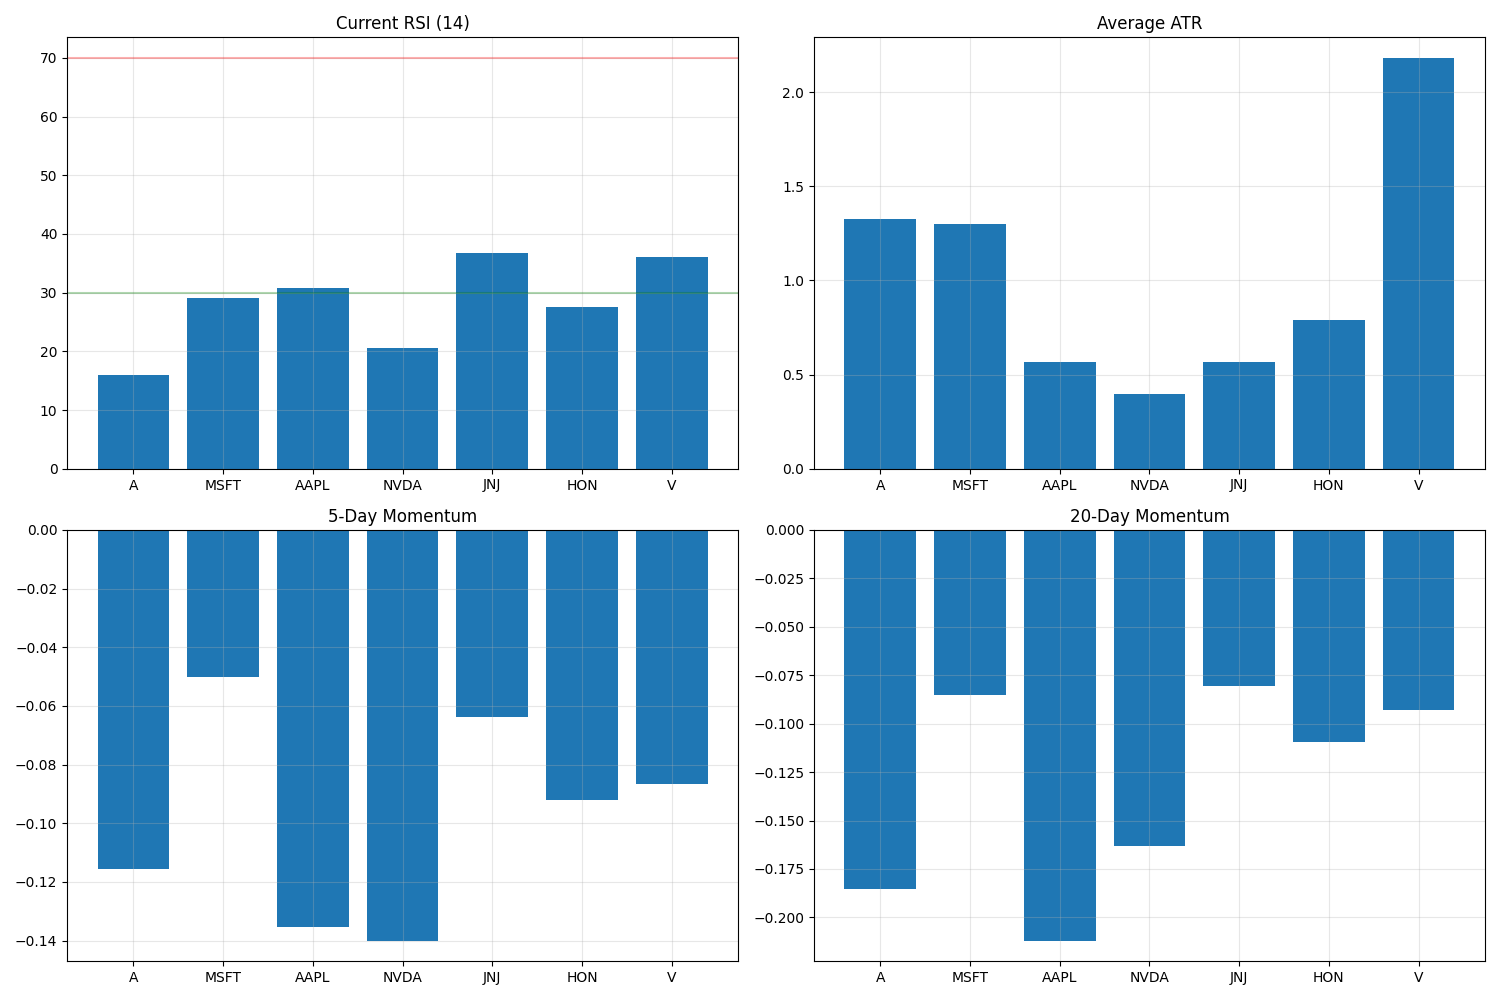
\includegraphics[width=1.25\textwidth]{stocktechs.png}}
    \caption{RSI, ATR, 5-Day Momentum, and 20-Day Momentum for all seven stock tickers used in project}
    \label{fig:1}
\end{figure}
\begin{figure}[H]
    \centering
    \makebox[\textwidth][c]{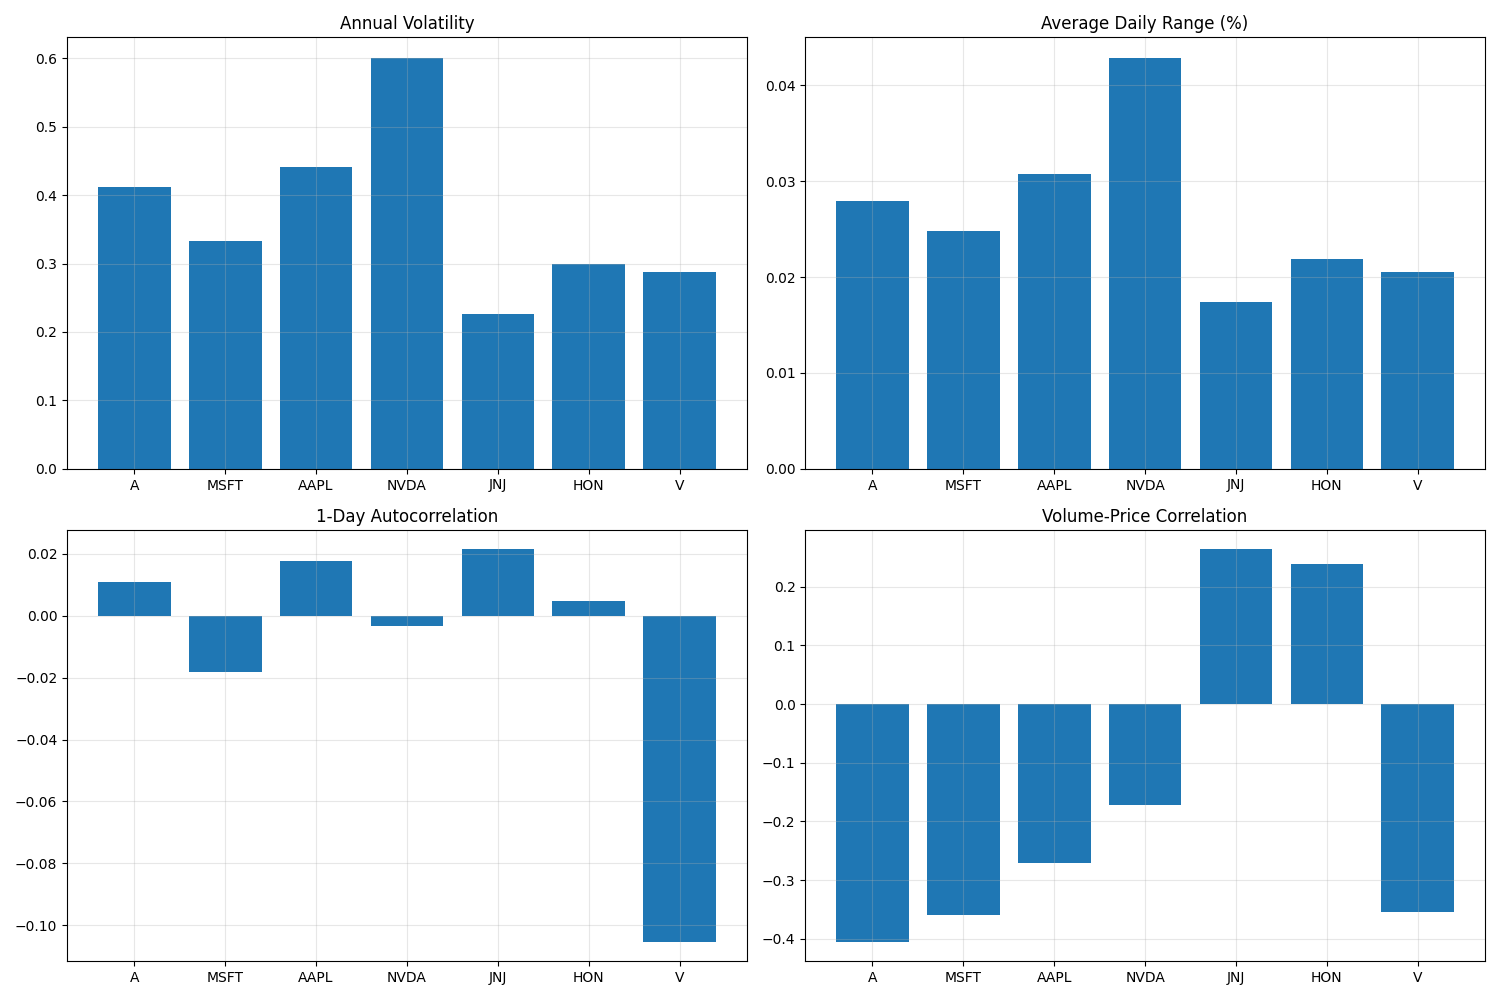
\includegraphics[width=1.25\textwidth]{stockmets.png}}
    \caption{Volatility, ADR, Autocorrelation, and VP-Correlation metrics for additional feature selection support}
    \label{fig:2}
\end{figure}
\subsection*{Model Training and Prediction}
The model is trained using Qiskit's \gls{qsvc} function which is the updated version of the \gls{qsvm} function that has since been deprecated. The \gls{qsvc} function requires many variables to be set up prior to running. First, a feature map must be created in order to represent the data in a quantum fashion. We must encode the classical bits that represent each feature into qubits, to do this we use qiskit's ZZFeatureMap function. This function creates a second-order Pauli-Z evolution circuit (See Fig.3) which encodes each x parameter (representing the features selected) into a qubit. This means that we can encode any amount of features selected into the same amount of qubits. The amount of qubits is directly correlated with the increase in processing time and decrease of accuracy, therefore we must be careful when navigating this issue. 
The solutions we determined is later discussed in the results section. 
\begin{figure}[H]
    \centering
    \makebox[\textwidth][c]{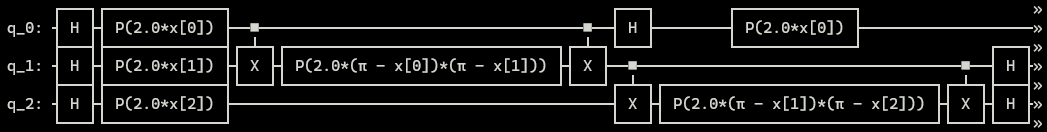
\includegraphics[width=1.25\textwidth]{zzfeature.png}}
    \caption{ZZFeatureMap Encoding Three Qubits}
    \label{fig:3}
\end{figure}
\section{Results}
After the feature map is created a qiskit StateVectorSampler is initialized that simulates the training of the \gls{qsvc} classifier, this is done instead of using a real quantum computer as the project does not incorporate a high order of qubits which would require more processing power. Using the qiskit-machine-learning library we generate a FidelityQuantumKernel which is used to map the data that has now passed through the ZZFeatureMap into a higher dimensional space. This allows for the non-linearly separable data to instead be linearly separable. When some data is unable to be separated linearly, we can add in a z-axis, and then have the potential to "slice" this data through a third dimension which then allows it to be linearly separable where previously was not possible (See Fig.4). 
\begin{figure}[H]
    \centering
    \makebox[\textwidth][c]{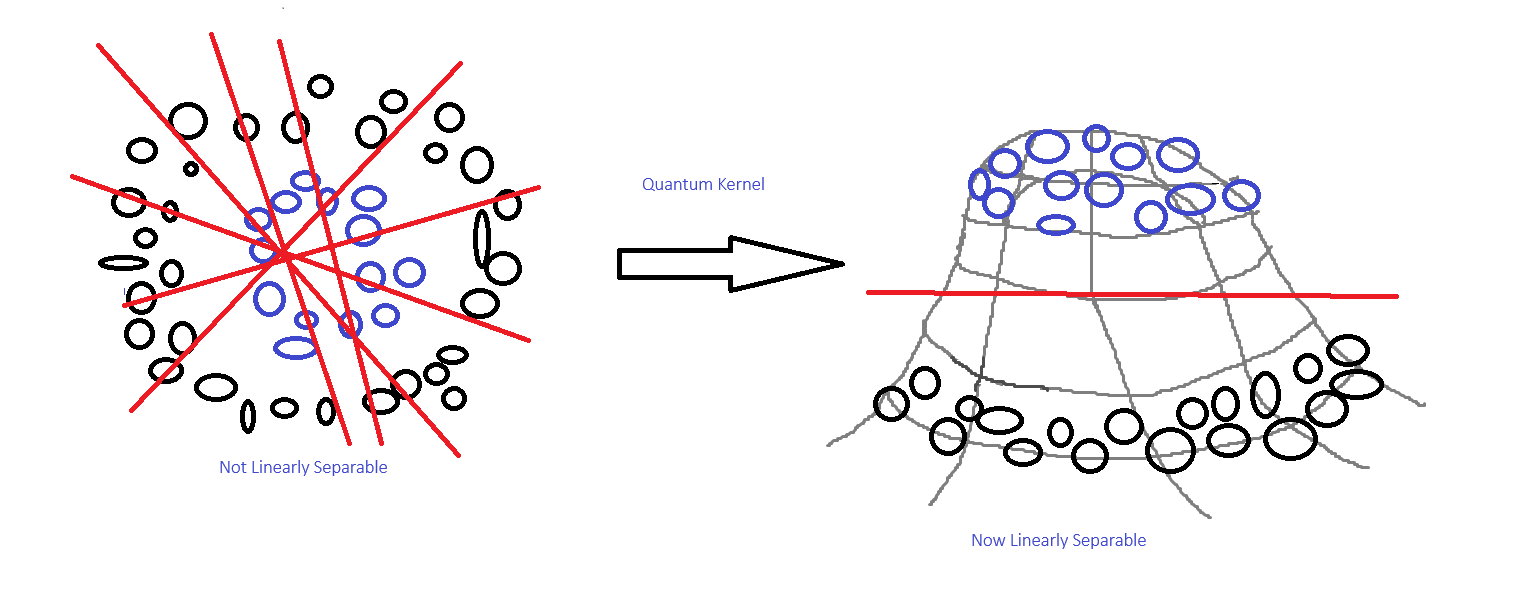
\includegraphics[width=1.25\textwidth]{quantumkernel.png}}
    \caption{Quantum Kernel classifies blue data and black data from non-linearly separable two-dimensional space (left) into linearly separable three-dimensional space (right)}
    \label{fig:4}
\end{figure}
\noindent
Once the feature map, sampler, and quantum kernel are prepared, then the \gls{qsvc} can be initialized. It uses the quantum kernel and a variable C as the parameters. This C value represents the red line in Figure 3. A larger C value will create a larger minimum margin for the line, which means it will be closer towards the blue data, a lower c will make the red line farther towards the black data. The value of C is purely dependent on how the data looks, if there are a presence of outliers on one or the other side, then the value of C can be changed to get a better representation of all the data. 
\section{Evaluation}
The study in which we are comparing our model tested many different models and dimensionality reduction algorithms to attempt to find the optimal combination. The highest average accuracy and f-score value they were able to achieve was 60.26\% and 62.24\% respectively. This was done with a classical machine learning model using a Quantum Annealing algorithm with 5 qubits. The highest \gls{qsvm} metrics were achieved with the Principal Component Analysis algorithm and 5 qubits. This resulted in 56.58\% accuracy and 59.79\% f-score. We will be using these values as our goals to achieve. Testing was done on different hyperparameters in order to determine what would lead to the optimal prediction metrics. The interchangeable areas of the software during testing was the features, the number of repetitions of the ZZFeatureMap on the circuit, the C-value of the \gls{qsvm}, and the entanglement scheme of the ZZFeatureMap.
\\
\\
Out of all previously mentioned hyperparameters, only one had little effect on the end outcome. The C-value of the \gls{qsvm} was only changed once throughout all testing, from 10.0 to 5.0, and optimality was found with the 5.0 C-value. Therefore we determined this parameter to be insignificant when determining optimal accuracy and f-score. For the other parameters, we had tested each at different values until we reach outcomes better than the ones found in the comparative study. To test the features and their performance, we began with a baseline test over a single feature combination, this involved combining two raw data columns (previous close and volume) directly from the dataset. This was the simplest combination that would still allow the model to learn based on the stock metrics determined prior. Starting with this combination allowed us to view the general trends of each of the other hyperparameters, and changing them will affect either the runtime or the outcome of the model. 
\begin{figure}[H]
    \centering
    \makebox[\textwidth][c]{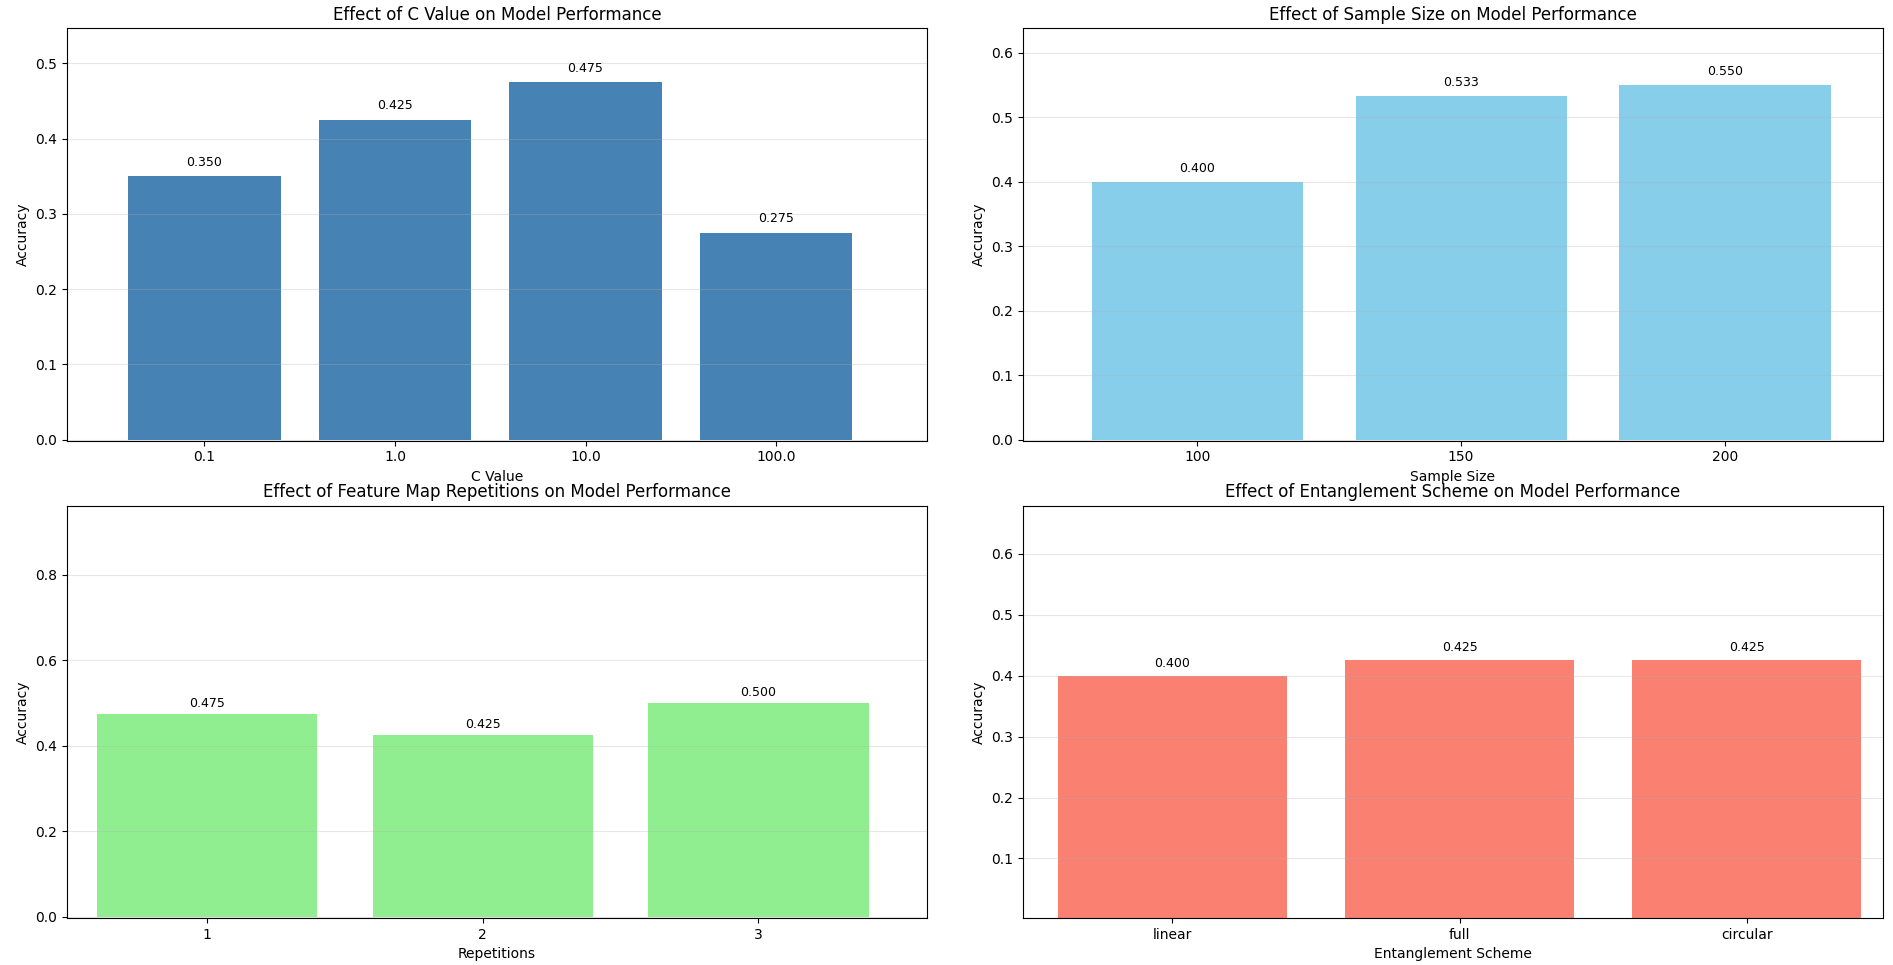
\includegraphics[width=1.25\textwidth]{baselinetest.png}}
    \caption{Baseline tests on feature combination (Previous Close,Volume) at different sample sizes, entanglement schemes, C values, and circuit repetitions}
    \label{fig:5}
\end{figure}
\noindent
Based of the results, we determined that effect on run-time was far more significant than the changes to the accuracy. Changes in sample size resulted in the program running anywhere from 2 minutes to 15 minutes, the effect of sample size on the runtime seemed to be exponential. We set the general testing sample size to 200 to ensure that the tests would not take too long, and so that we would get a good representation of training and testing data (160 train, 40 test) Repetitions and entanglement schemes also had similar effects on the runtime but not to the degree that the sample size had. In terms of the effect on the accuracy, none had significant effects other than C-value, which was significantly lower at 0.1 and at 100.0. This is due to the effect that the C-value has on margin for the hyperplane, which most likely caused a significant amount of errors to occur in training. The optimal area for the C value was determined to be somewhere in between 1.0 and 10.0, we decided it to be 5.0. For repetitions and entanglement scheme, we began with using 1 and full, however this was changed later due to the circuit complexity becoming too great. Since the change in accuracy values were insignificant on repetitions and entanglement, this meant we could change them freely without much consequence. 
\\
\\
Now that the optimal hyperparemeters were determined, the most importance task of feature selection was needed to be done. This required testing multiple different possible feature combinations until we found a combination that outperformed the highest average accuracy and f-score of the study we are comparing with. There is two measures that are important for feature selection; number of features (qubits) and the type of combination. In order to achieve an outperforming prediction model we needed to find the proper amount of qubits so that the circuit was not too complex and thus result in excessive noise, as well as find the right combination of features to ensure we are covering every type of stock trend. From the metrics in figure 1 and 2 we determined that volume, momentum, volatility are all important markers for these stocks, these will be the key factors to test in order to help predict the trends optimally. 
The first set of tests were done in order to correlate the highest outcomes with specific indicators, if one particular indicator was linked to multiple instances of high performance, then that indicator was determined to be ideal. 
\begin{figure}[H]
    \centering
    \makebox[\textwidth][c]{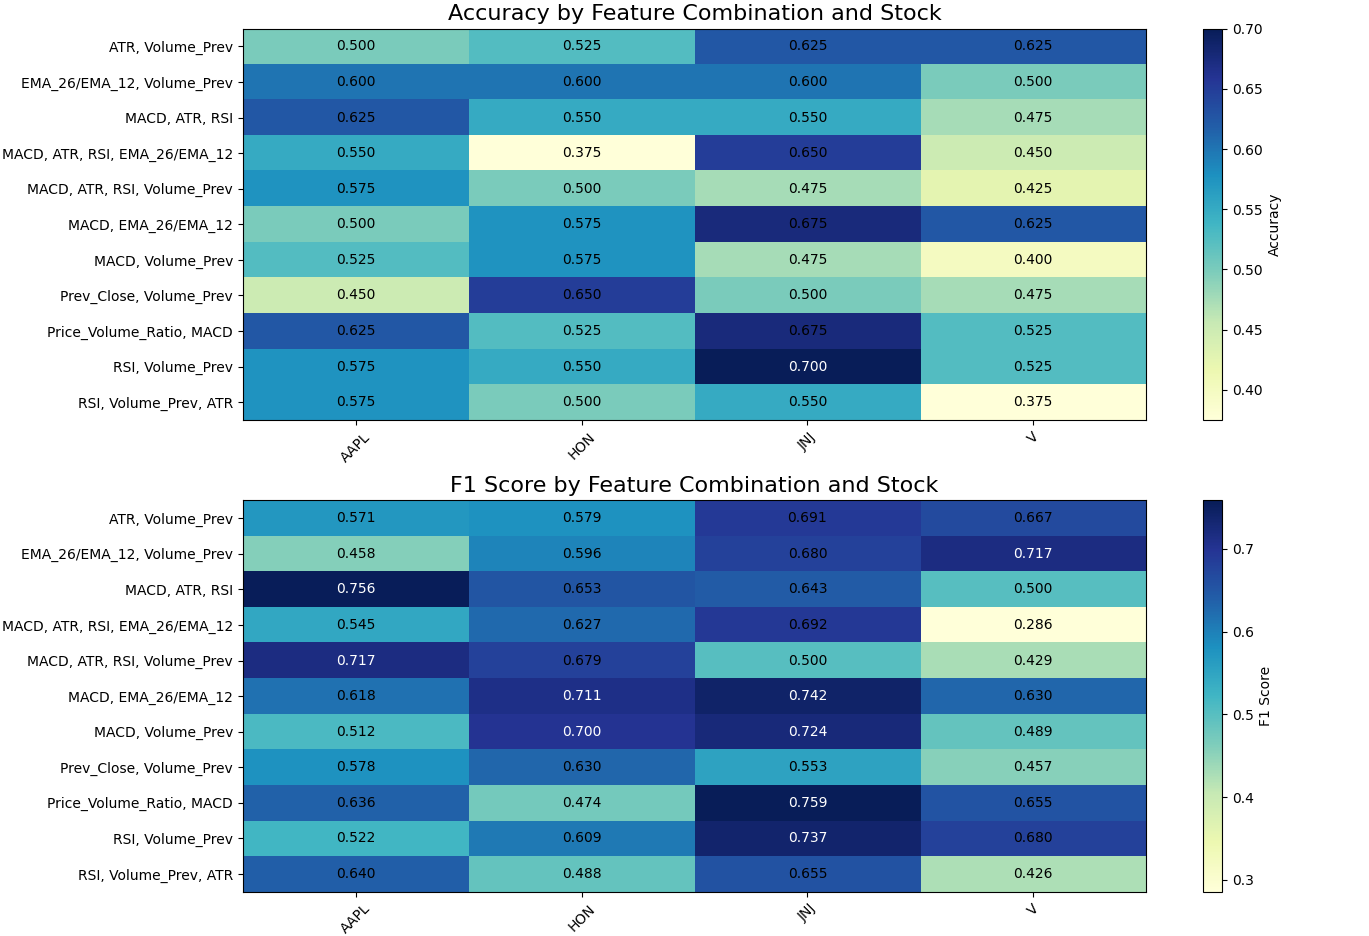
\includegraphics[width=1.25\textwidth]{firsttestlinear.png}}
    \caption{Initial tests on correlation between featrure combinations and (f1 score, accuracy)}
    \label{fig:6}
\end{figure}
\noindent
\begin{figure}[H]
    \centering
    \makebox[\textwidth][c]{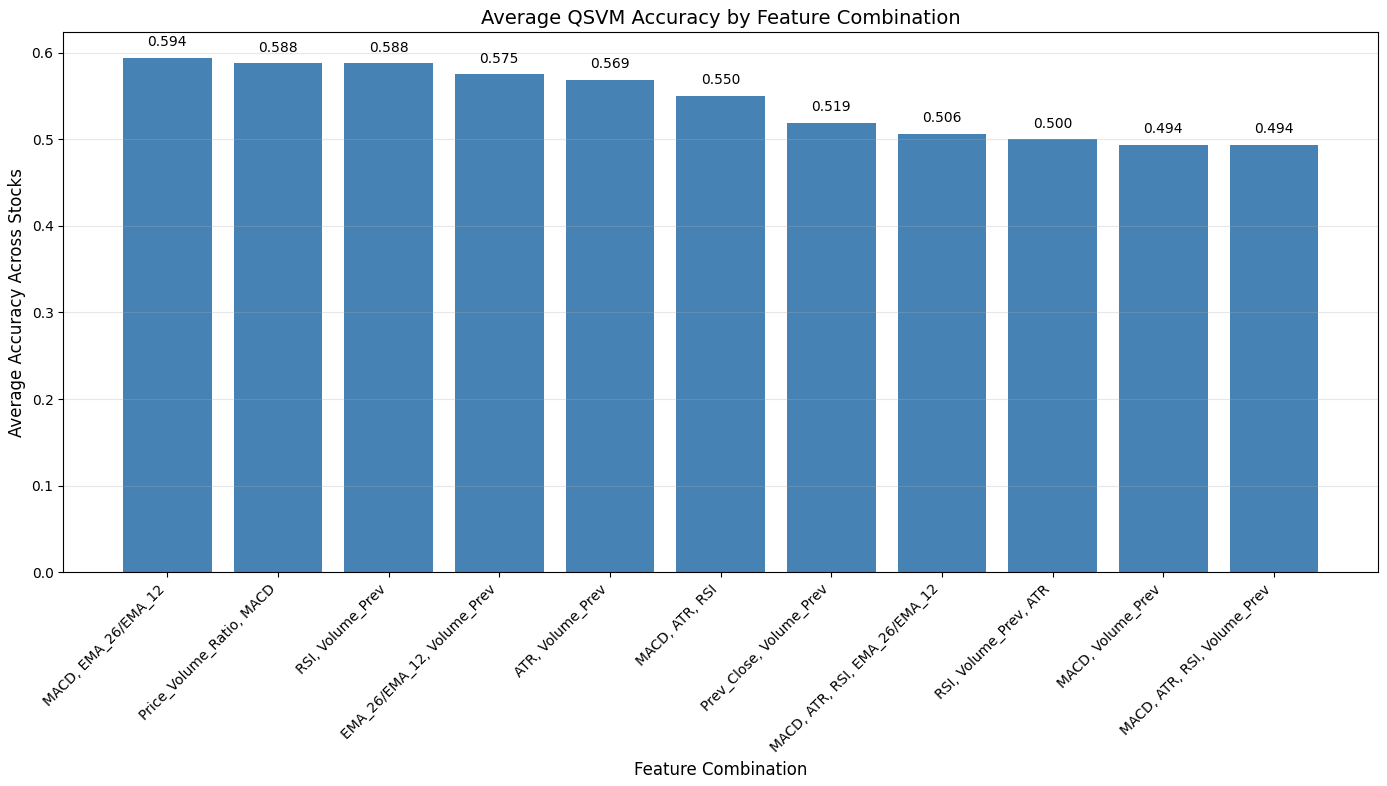
\includegraphics[width=1.25\textwidth]{firsttestbars.png}}
    \caption{Average accuracy of different feature combinations throughout all stock predictions}
    \label{fig:7}
\end{figure}
\noindent
The first tests helped determine the indicators that seemed to perform better than others. We found that feature combinations of more then 2 resulted in lower average accuracy (See figure 7),
therefore it was optimal to pick just two features to ensure accuracy remained highest. The choices of features were based on utlizing more stock indicators instead of raw data,
in this way we could determine which of the specific indicators has more of a presence in high performing \gls{qsvm} predictions. The first tests also proved to be promising as we noticed that most feature combination choices 
at minimum replicated withing 3-5\% of the average scores found in the paper. The highest performing feature combination of (\gls{macd}) and the \gls{ema} Ratio (\gls{ema}26/\gls{ema}12), was able to outperform the average 
average accuracy and average f1-score of the highest \gls{qsvm} implemented in the paper. The \gls{qsvm} with Principal Component Analysis and 5 features achieved an accuracy of 56.58\% and f-score of 
59.79\% while our implementation of the \gls{qsvm} achieved an accuracy of 59.4\% and f-score of 67.5\%. 
\\
\\
The difference in sectors among the stocks chosen provided the \gls{qsvm} with learning data that has wildly different patterns. This was demonstrated in the testing when looking at the 
performance of feature combinations for specific stocks. With the chosen feature combinations, a C-value of 5.0, 2 repetitions of the ZZFeatureMap, and linear entanglement, we were 
able to produce a \gls{qsvm} that outperformed the paper on every metric (except for HON f-score) for each different stock (See figure 8). These difference was much greater than the difference present in the average accuracy and f1-score 
value. They do not hold as much weight as the total average accuracy and f1-score values do, nonetheless it is still very notable for this project. 
\begin{figure}[H]
    \centering
    \makebox[\textwidth][c]{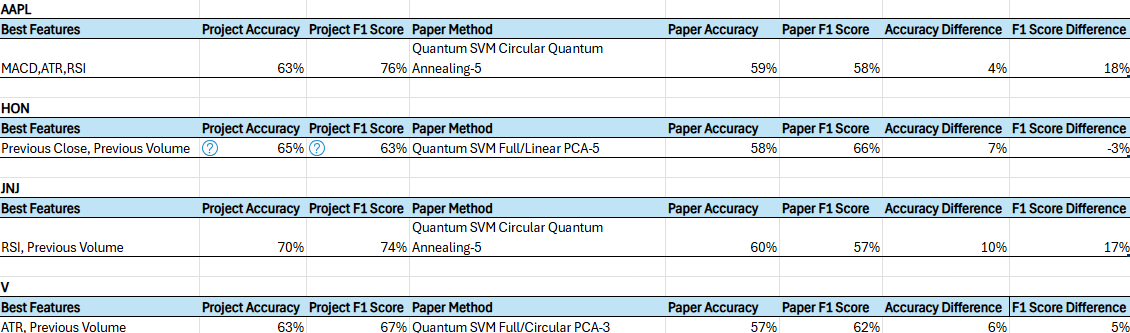
\includegraphics[width=1.25\textwidth]{firsttesttable.png}}
    \caption{Table demonstrating comparison of our \gls{qsvm} with specific feature combinations vs. paper's \gls{qsvm} model on predicting specific stocks}
    \label{fig:8}
\end{figure}
\noindent
\section{Conclusion}
\subsection{Summary}
The complexity of predicting stock prices using quantum algorithms and methods remains a challenge. The overwhelming unpredictability that 
the stock market poesses makes such a task very difficult. The results from this project aim to give details on methods to further optimize
the usage of \gls{qsvm}'s in such a binary classification problem. This project revealed the grave importance of testing different parameters in order to 
develop further optimizations, especially related to the usage of features in the \gls{qsvm}. 
\subsection{Relevance}
The content of this project is particularly relevant to the course as it involves heavily with developed further optimized structure in a quantum fashion 
to achieve a goal. The ability to transform a difficult classical issue into a easier quantum one has been the forefront of the course since it began. 
The optimization towards stock price prediction sheds light on the both the ability that quantum computers have in binary classification, and the potential 
for greater limits in the field. 
\subsection{Future Work}
For this project in particular, many improvements can be made in order to develop this into higher optimality. Developement of a 
feature selection algorithm that allows for dimensionality reduction while maintaining the mathematically most optimal features is something 
that could be incorporated in the future. The inclusion of real quantum computers is another topic that could be developed in the future. Utilizing IBM's real quantum computer
could have the processing capabilities to predict stock prices with many more qubits that we were able to simulate, leading to further developements towards a better model. 
\section*{Contribution of Team Members}
\subsection*{Code Implementation}
A. Benjamin Muir implemented the Feature Map, main \gls{qsvm} functionality, and data testing variant of Code
\\
\noindent
B. Hasan Fakih implemented the stock indicator helper functions, model training and testing
\\
\noindent
C. Both members worked equally on the data pre-processing/preperation of data  
\subsection*{Report}
A. Benjamin Muir worked on Results, Evaluation and Conclusion 
\\
\noindent
B. Hasan Fakih worked on Introduction and Background Information
\\
C. Benjamin Muir and Hasan Fakih both jointly worked on the reasearch and finding papers relevant to the project

\newpage

\begin{thebibliography}{99}
    \bibitem{Xia24} 
    Xia, S., Wei, M., Zhu, Y., \& Pu, Y. (2024). AI-Driven Intelligent Financial Analysis: Enhancing Accuracy and Efficiency in Financial Decision-Making. Journal of Economic Theory and Business Management, 1(5), 1–11. https://doi.org/10.5281/zenodo.13926298

    \bibitem{Chhajer22} 
    Parshv Chhajer, Manan Shah, Ameya Kshirsagar,
    The applications of artificial neural networks, support vector machines, and long–short term memory for stock market prediction,
    Decision Analytics Journal,
    Volume 2,
    2022,
    100015,
    ISSN 2772-6622,
    https://doi.org/10.1016/j.dajour.2021.100015

    \bibitem{muir2025}
    Alexander, A., \& Widdows, D. (2022). Quantum text encoding for classification tasks. 2022 IEEE/ACM 7th Symposium on Edge Computing (SEC), 355 – 361. https://doi.org/10.1109/sec54971.2022.00052 

    \bibitem{bhasin2024}
    Bhasin, N. K., Kadyan, S., Santosh, K., HP, R., Changala, R., \& Bala, B. K. (2024). Enhancing quantum machine learning algorithms for optimized financial portfolio management. 2024 Third International Conference on Intelligent Techniques in Control, Optimization and Signal Processing (INCOS), 1 – 7. https://doi.org/10.1109/incos59338.2024.10527612 

    \bibitem{onyshchak2020}
    Onyshchak, O. (2020, April 2). Stock market dataset. Kaggle. https://www.kaggle.com/datasets/jacksoncrow/stock-market-dataset/data 

    \bibitem{srivastava2023}
    Srivastava, N., Belekar, G., Shahakar, N., \& Babu H., A. (2023). The potential of quantum techniques for stock price prediction. 2023 IEEE International Conference on Recent Advances in Systems Science and Engineering (RASSE), 1 – 7. https://doi.org/10.1109/rasse60029.2023.10363533
    
\end{thebibliography}

\newpage

\glsaddall
\printglossaries

\end{document}
